\section{Chapter 1}

\begin{figure}[H]
	\centering
	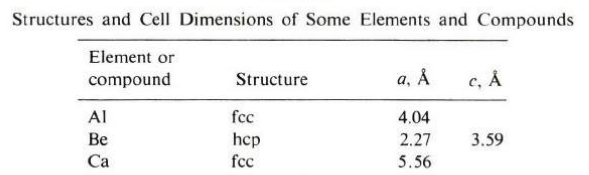
\includegraphics[width=0.7\linewidth]{Graphics/Chapter1/StructuresAndCellDimension_Table1_2_Omar}
	\caption{}
	\label{}
\end{figure}


\textbf{Unit Cell}
\begin{figure}[H]
	\centering
	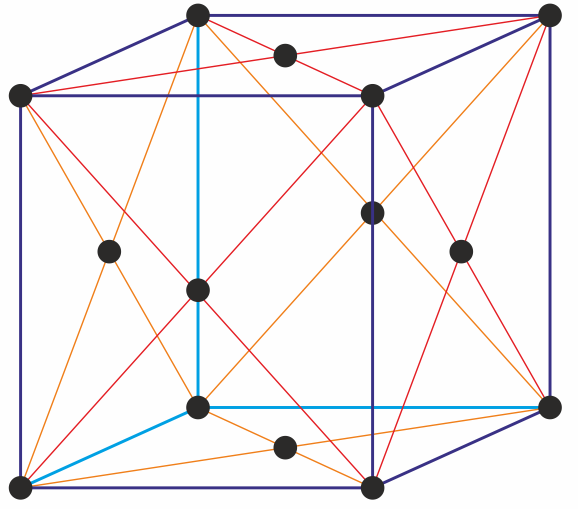
\includegraphics[width=0.4\linewidth]{Graphics/Chapter1/face-centered_cubic_lattice.png}
	\caption{}
	\label{}
\end{figure}

\textbf{Primitive Vectors}

\textbf{Packaging Factor}

The Packaging Factor can be calculated as the ratio between the
volume of the atoms in the unit cell to the volume of the unit cell.

The volume of the unit cell can be calculated as:

$$V_{UC} = a^3$$

The unit cell containts 4 whole atoms 

The relationship between the parameter $a$ and the radius of the Radius of the atomic sphere is given as:
$$r = \frac{\sqrt{2}}{4} a $$

$$APF = \frac{\pi}{3 \cdot \sqrt{2}} \approx 74\%$$


\textbf{Density}

The atomic mass of calcium us given as:
$$M_{Ca} = 40.078 \frac{g}{mol}$$

$$\rho = \frac{4}{N_A} \cdot \frac{M_{Ca}}{V_{UC}} = 1.55 \frac{g}{cm^3}$$

\textbf{Linear Density [110]}
